%! Tex program = lualatex
\documentclass{beamer}
\usepackage{amsfonts,amsmath,oldgerm}
%%custom
\usepackage{graphicx}
\usepackage{float}
\usepackage[siunitx, american, cute inductors]{circuitikz} % Circuitos
\usepackage{caption} % Legenda nas figuras
\usepackage{siunitx} %unidade no SI
\usepackage{amssymb}
\usepackage{xcolor}
\usepackage{colortbl} %colorir tabela
%%endcustom
% Para justificar o texto
\usepackage{ragged2e}
\justifying

%para o cronograma
\usepackage{multirow}
%para códigos
\usepackage{minted}
\usepackage{multirow}
\usepackage{subcaption} %permite o aninhamento de imagens

\apptocmd{\frame}{}{\justifying}{} % Allow optional arguments after frame.

\usetheme{sintef}

\newcommand{\testcolor}[1]{\colorbox{#1}{\textcolor{#1}{test}}~\texttt{#1}}

\usefonttheme[onlymath]{serif}

\titlebackground*{assets/background}

\newcommand{\hrefcol}[2]{\textcolor{cyan}{\href{#1}{#2}}}

\title{Tittle}
\subtitle{Subtittle}
\author{
\textbf{Fulano de Souza}\quad
\textbf{Joe Ferreira Scholtz} \newline
\textbf{Ciclano da Silva}
}
\date{Jan 2000}

\toctittle{Table of Contents}


\begin{document}
\maketitle

\section{Introduction}

\begin{frame}{Slide tittle}

\end{frame}


\section{Planta}


\begin{frame}{Proposta}

\begin{columns}
    \begin{column}{0.5\textwidth}
        \begin{figure}[htbp]
            \centering
            \resizebox{0.8\textwidth}{!}{


\tikzset{every picture/.style={line width=0.75pt}} %set default line width to 0.75pt        

\begin{tikzpicture}[x=0.75pt,y=0.75pt,yscale=-1,xscale=1]
%uncomment if require: \path (0,682); %set diagram left start at 0, and has height of 682

%Image [id:dp0791029514129229] 
\draw (390,240) node  {\includegraphics[width=315pt,height=300pt]{tikz/modelo/modelo.png}};
%Straight Lines [id:da12694700194316932] 
\draw [color={rgb, 255:red, 189; green, 16; blue, 224 }  ,draw opacity=1 ][line width=3.75]    (220,125) -- (390,125) -- (390,145) -- (310,145) -- (310,220) -- (564,220) ;
\draw [shift={(570,220)}, rotate = 180] [color={rgb, 255:red, 189; green, 16; blue, 224 }  ,draw opacity=1 ][line width=3.75]    (25.14,-7.57) .. controls (15.99,-3.21) and (7.61,-0.69) .. (0,0) .. controls (7.61,0.69) and (15.99,3.21) .. (25.14,7.57)   ;
%Straight Lines [id:da29542059738648274] 
\draw [color={rgb, 255:red, 126; green, 211; blue, 33 }  ,draw opacity=1 ][line width=3.75]    (220,130) -- (385,130) -- (385,140) -- (305,140) -- (305,225) -- (305,399) ;
\draw [shift={(305,405)}, rotate = 270] [color={rgb, 255:red, 126; green, 211; blue, 33 }  ,draw opacity=1 ][line width=3.75]    (25.14,-7.57) .. controls (15.99,-3.21) and (7.61,-0.69) .. (0,0) .. controls (7.61,0.69) and (15.99,3.21) .. (25.14,7.57)   ;

% Text Node
\draw (225,85) node  [font=\large] [align=left] {\begin{minipage}[lt]{41.14pt}\setlength\topsep{0pt}
\begin{center}
SF
\end{center}

\end{minipage}};
% Text Node
\draw (305,85) node  [font=\large] [align=left] {\begin{minipage}[lt]{41.14pt}\setlength\topsep{0pt}
\begin{center}
RB
\end{center}

\end{minipage}};
% Text Node
\draw (455,130) node  [font=\large] [align=left] {\begin{minipage}[lt]{41.14pt}\setlength\topsep{0pt}
\begin{center}
PM1
\end{center}

\end{minipage}};
% Text Node
\draw (235,250) node  [font=\large] [align=left] {\begin{minipage}[lt]{41.14pt}\setlength\topsep{0pt}
\begin{center}
DS
\end{center}

\end{minipage}};
% Text Node
\draw (235,410) node  [font=\large] [align=left] {\begin{minipage}[lt]{41.14pt}\setlength\topsep{0pt}
\begin{center}
XS1
\end{center}

\end{minipage}};
% Text Node
\draw (550,270) node  [font=\large] [align=left] {\begin{minipage}[lt]{41.14pt}\setlength\topsep{0pt}
\begin{center}
XS2
\end{center}

\end{minipage}};
% Text Node
\draw (390,320) node  [font=\large] [align=left] {\begin{minipage}[lt]{41.14pt}\setlength\topsep{0pt}
\begin{center}
PM2
\end{center}

\end{minipage}};


\end{tikzpicture}}
            \caption{Planta para a máquina de \textit{milkshake}.}
            \label{fig:sistema}
        \end{figure}
    \end{column}
    \begin{column}{0.5\textwidth}
        \begin{figure}[htbp]
            \centering
            \begin{minipage}{\textwidth}
                \centering
                \resizebox{0.2\textwidth}{!}
                {


\tikzset{every picture/.style={line width=0.75pt}} %set default line width to 0.75pt        


\begin{tikzpicture}[x=0.75pt,y=0.75pt,yscale=-1,xscale=1]
%uncomment if require: \path (0,300); %set diagram left start at 0, and has height of 300

%Curve Lines [id:da33623388382234665] 
\draw [draw opacity=0][fill={rgb, 255:red, 255; green, 255; blue, 255 }  ,fill opacity=1 ][line width=0.75] [line join = round][line cap = round]   (215.8,98.12) .. controls (218.97,99.2) and (223.27,104.03) .. (225.3,101.37) .. controls (233.8,85.17) and (240.3,71.17) .. (245.55,59.12) .. controls (246.45,55.63) and (240.48,48.25) .. (238.3,51.12) .. controls (231.05,62.67) and (223.63,82.12) .. (216.3,97.62) ;
%Curve Lines [id:da6517219999182808] 
\draw [draw opacity=0][fill={rgb, 255:red, 255; green, 255; blue, 255 }  ,fill opacity=1 ][line width=0.75] [line join = round][line cap = round]   (238.05,50.92) .. controls (240.3,47.42) and (242.78,43.66) .. (246.3,44.17) .. controls (250.56,44.78) and (253.17,49.68) .. (255.3,53.42) .. controls (260.05,64.42) and (263.3,71.17) .. (270.5,85.92) .. controls (271.08,88.99) and (264.5,94.12) .. (262.55,91.67) .. controls (257.55,81.17) and (253.55,70.92) .. (247.05,57.42) .. controls (248.05,54.67) and (245.56,60.93) .. (244.3,60.42) .. controls (240.76,58.98) and (235.84,54.58) .. (237.55,51.17) ;
%Curve Lines [id:da33392627803622843] 
\draw [draw opacity=0][fill={rgb, 255:red, 208; green, 2; blue, 27 }  ,fill opacity=1 ][line width=0.75] [line join = round][line cap = round]   (268.05,81.17) .. controls (268.3,84.17) and (267.16,87.64) .. (268.8,90.17) .. controls (268.58,91.42) and (272.58,88.17) .. (268.8,82.17) ;
%Curve Lines [id:da05524754410677479] 
\draw [draw opacity=0][fill={rgb, 255:red, 208; green, 2; blue, 27 }  ,fill opacity=1 ][line width=0.75] [line join = round][line cap = round]   (259.05,63.42) .. controls (258.72,69.83) and (259.8,76.92) .. (258.8,81.67) .. controls (259.03,83.74) and (261.29,89.69) .. (261.8,87.67) .. controls (263.05,71.42) and (264.52,72.32) .. (260.05,64.67) ;
%Curve Lines [id:da10288432289609939] 
\draw [draw opacity=0][fill={rgb, 255:red, 208; green, 2; blue, 27 }  ,fill opacity=1 ][line width=0.75] [line join = round][line cap = round]   (252.3,47.92) .. controls (251.97,54.33) and (252.08,60.5) .. (252.05,66.17) .. controls (252.28,68.24) and (254.54,74.19) .. (255.05,72.17) .. controls (256.3,55.92) and (256.58,55.75) .. (253.3,49.17) ;
%Curve Lines [id:da48052459184272034] 
\draw [draw opacity=0][fill={rgb, 255:red, 208; green, 2; blue, 27 }  ,fill opacity=1 ][line width=0.75] [line join = round][line cap = round]   (221.25,85.67) .. controls (224.21,82.88) and (241.33,71.42) .. (235.5,80.67) .. controls (234.33,83.17) and (233.79,85.72) .. (231.75,87.17) .. controls (228,87.33) and (219.5,95.83) .. (215,99.33) .. controls (215.5,96.83) and (220.33,87.5) .. (222.25,84.17) ;
%Curve Lines [id:da5565878074443247] 
\draw [draw opacity=0][fill={rgb, 255:red, 208; green, 2; blue, 27 }  ,fill opacity=1 ][line width=0.75] [line join = round][line cap = round]   (237.8,53.17) .. controls (242.05,49.83) and (244.3,46.33) .. (251.3,45.92) .. controls (251.8,46.33) and (247.55,43.83) .. (246.3,44.17) .. controls (240.55,46.08) and (239.3,50.33) .. (238.55,52.42) ;
%Curve Lines [id:da38187296164180884] 
\draw [draw opacity=0][fill={rgb, 255:red, 208; green, 2; blue, 27 }  ,fill opacity=1 ][line width=0.75] [line join = round][line cap = round]   (232.8,62.42) .. controls (235.76,59.63) and (242.05,54.58) .. (247.05,57.42) .. controls (245.55,57.33) and (245.34,62.47) .. (243.3,63.92) .. controls (239.55,64.08) and (231.05,72.58) .. (226.55,76.08) .. controls (227.05,73.58) and (231.88,64.25) .. (233.8,60.92) ;
%Shape: Ellipse [id:dp40094882673661036] 
\draw  [draw opacity=0][line width=2.25]  (150.84,195.84) .. controls (152.87,183.77) and (177.58,177.86) .. (206.03,182.64) .. controls (234.48,187.43) and (255.9,201.08) .. (253.87,213.15) .. controls (251.84,225.22) and (227.14,231.12) .. (198.69,226.34) .. controls (170.24,221.56) and (148.82,207.9) .. (150.84,195.84) -- cycle ;
%Straight Lines [id:da8992804145996609] 
\draw [color={rgb, 255:red, 74; green, 74; blue, 74 }  ,draw opacity=1 ][fill={rgb, 255:red, 155; green, 155; blue, 155 }  ,fill opacity=1 ]   (238.5,49.67) -- (215.5,98.42) ;
%Straight Lines [id:da1621651244646496] 
\draw [color={rgb, 255:red, 74; green, 74; blue, 74 }  ,draw opacity=1 ]   (245.5,59.67) -- (225.5,101.67) ;
%Shape: Arc [id:dp8497438534326236] 
\draw  [draw opacity=0][fill={rgb, 255:red, 252; green, 52; blue, 74 }  ,fill opacity=1 ][line width=2.25]  (237.99,121.53) .. controls (235.96,133.6) and (212.65,139.74) .. (185.92,135.25) .. controls (159.19,130.76) and (139.17,117.33) .. (141.2,105.27) .. controls (143.23,93.2) and (166.54,87.06) .. (193.27,91.55) .. controls (219.99,96.04) and (240.02,109.47) .. (237.99,121.53) -- (189.59,113.4) -- cycle ; \draw  [draw opacity=0][line width=2.25]  (237.99,121.53) .. controls (235.96,133.6) and (212.65,139.74) .. (185.92,135.25) .. controls (159.19,130.76) and (139.17,117.33) .. (141.2,105.27) .. controls (143.23,93.2) and (166.54,87.06) .. (193.27,91.55) .. controls (219.99,96.04) and (240.02,109.47) .. (237.99,121.53) -- cycle ;  
%Curve Lines [id:da6745169594181273] 
\draw [draw opacity=0][fill={rgb, 255:red, 201; green, 195; blue, 195 }  ,fill opacity=0.66 ][line width=0.75] [line join = round][line cap = round]   (141.2,105.27) .. controls (141.2,97.28) and (140.21,80.26) .. (145.2,75.27) .. controls (148.96,71.51) and (157.13,71.28) .. (163.2,70.27) .. controls (189.71,65.85) and (220.53,70.6) .. (235.2,85.27) .. controls (238.08,88.15) and (244.66,90.38) .. (245.2,95.27) .. controls (246.45,106.56) and (240.2,111.49) .. (240.2,121.27) .. controls (240.2,122.47) and (239.05,119.12) .. (238.2,118.27) .. controls (236.27,116.33) and (236.04,111.11) .. (234.2,109.27) .. controls (230.27,105.34) and (213.56,95.86) .. (208.2,95.27) .. controls (191.63,93.43) and (186.78,90.4) .. (164.2,91.27) .. controls (159.82,91.44) and (153.98,93.67) .. (149.2,95.27) .. controls (145.95,96.35) and (144.7,103.27) .. (141.2,103.27) ;
%Shape: Trapezoid [id:dp9836029479786901] 
\draw  [draw opacity=0][fill={rgb, 255:red, 252; green, 52; blue, 74 }  ,fill opacity=1 ] (238.5,125.93) -- (205.79,237.18) -- (139.82,223.54) -- (142.27,106.04) -- cycle ;
%Shape: Arc [id:dp10237578178410933] 
\draw  [draw opacity=0][line width=2.25]  (142.83,83.67) .. controls (142.83,83.67) and (142.83,83.67) .. (142.83,83.67) .. controls (144.85,71.6) and (169.56,65.69) .. (198.01,70.48) .. controls (226.46,75.26) and (247.88,88.91) .. (245.85,100.98) -- (194.34,92.32) -- cycle ; \draw  [line width=2.25]  (142.83,83.67) .. controls (142.83,83.67) and (142.83,83.67) .. (142.83,83.67) .. controls (144.85,71.6) and (169.56,65.69) .. (198.01,70.48) .. controls (226.46,75.26) and (247.88,88.91) .. (245.85,100.98) ;  
%Shape: Ellipse [id:dp926473623529513] 
\draw  [line width=2.25]  (139.48,224.75) .. controls (140.18,220.59) and (155.52,219.7) .. (173.76,222.76) .. controls (191.99,225.82) and (206.21,231.68) .. (205.51,235.85) .. controls (204.81,240.01) and (189.46,240.9) .. (171.22,237.84) .. controls (152.99,234.77) and (138.78,228.91) .. (139.48,224.75) -- cycle ;
%Shape: Ellipse [id:dp042692779544714066] 
\draw  [fill={rgb, 255:red, 252; green, 52; blue, 74 }  ,fill opacity=1 ][line width=2.25]  (139.48,224.75) .. controls (140.18,220.59) and (155.52,219.7) .. (173.76,222.76) .. controls (191.99,225.82) and (206.21,231.68) .. (205.51,235.85) .. controls (204.81,240.01) and (189.46,240.9) .. (171.22,237.84) .. controls (152.99,234.77) and (138.78,228.91) .. (139.48,224.75) -- cycle ;
%Straight Lines [id:da7389947599407996] 
\draw [line width=2.25]    (139.48,224.75) -- (142.83,83.67) ;
%Straight Lines [id:da9728249678309886] 
\draw [line width=2.25]    (245.85,100.98) -- (205.51,235.85) ;
%Shape: Arc [id:dp3932843359864808] 
\draw  [draw opacity=0][fill={rgb, 255:red, 252; green, 52; blue, 74 }  ,fill opacity=1 ][line width=2.25]  (142.27,106.04) .. controls (144.3,93.97) and (167.61,87.83) .. (194.34,92.32) .. controls (221.07,96.82) and (241.09,110.24) .. (239.06,122.31) -- (190.67,114.17) -- cycle ; \draw  [line width=2.25]  (142.27,106.04) .. controls (144.3,93.97) and (167.61,87.83) .. (194.34,92.32) .. controls (221.07,96.82) and (241.09,110.24) .. (239.06,122.31) ;  
%Straight Lines [id:da8573053213137072] 
\draw [color={rgb, 255:red, 74; green, 74; blue, 74 }  ,draw opacity=1 ]   (248.75,60.17) -- (262.25,91.17) ;
%Straight Lines [id:da7298578047225213] 
\draw [color={rgb, 255:red, 74; green, 74; blue, 74 }  ,draw opacity=1 ]   (253.5,49.92) -- (270.5,85.92) ;
%Shape: Arc [id:dp15110507933656647] 
\draw  [draw opacity=0] (238.21,50.63) .. controls (240.06,46.83) and (242.88,44.41) .. (246.04,44.41) .. controls (248.99,44.41) and (251.65,46.53) .. (253.5,49.92) -- (246.04,61.41) -- cycle ; \draw  [color={rgb, 255:red, 74; green, 74; blue, 74 }  ,draw opacity=1 ] (238.21,50.63) .. controls (240.06,46.83) and (242.88,44.41) .. (246.04,44.41) .. controls (248.99,44.41) and (251.65,46.53) .. (253.5,49.92) ;  
%Shape: Arc [id:dp2274995624393623] 
\draw  [draw opacity=0] (245.1,60.59) .. controls (245.51,58.98) and (246.22,57.92) .. (247.03,57.92) .. controls (247.8,57.92) and (248.48,58.89) .. (248.89,60.38) -- (247.03,63.67) -- cycle ; \draw  [color={rgb, 255:red, 74; green, 74; blue, 74 }  ,draw opacity=1 ] (245.1,60.59) .. controls (245.51,58.98) and (246.22,57.92) .. (247.03,57.92) .. controls (247.8,57.92) and (248.48,58.89) .. (248.89,60.38) ;  
%Shape: Arc [id:dp4687377714663463] 
\draw  [draw opacity=0] (269.81,84.27) .. controls (269.81,84.27) and (269.81,84.27) .. (269.81,84.27) .. controls (271.3,86.15) and (270.71,89.09) .. (268.5,90.84) .. controls (266.29,92.59) and (263.3,92.49) .. (261.81,90.61) -- (265.81,87.44) -- cycle ; \draw  [color={rgb, 255:red, 74; green, 74; blue, 74 }  ,draw opacity=1 ] (269.81,84.27) .. controls (269.81,84.27) and (269.81,84.27) .. (269.81,84.27) .. controls (271.3,86.15) and (270.71,89.09) .. (268.5,90.84) .. controls (266.29,92.59) and (263.3,92.49) .. (261.81,90.61) ;  




\end{tikzpicture}}
                \subcaption{\textit{Milkshake} \textbf{sem} cobertura.}\label{fig:milk_00}
            \end{minipage}
            \begin{minipage}{\textwidth}
                \centering
                \resizebox{0.2\textwidth}{!}
                {


\tikzset{every picture/.style={line width=0.75pt}} %set default line width to 0.75pt        


\begin{tikzpicture}[x=0.75pt,y=0.75pt,yscale=-1,xscale=1]
%uncomment if require: \path (0,800); %set diagram left start at 0, and has height of 800

%Curve Lines [id:da7965757231260868] 
\draw [draw opacity=0][fill={rgb, 255:red, 255; green, 255; blue, 255 }  ,fill opacity=1 ][line width=0.75] [line join = round][line cap = round]   (202.6,412.72) .. controls (205.77,413.8) and (210.07,418.63) .. (212.1,415.97) .. controls (220.6,399.77) and (227.1,385.77) .. (232.35,373.72) .. controls (233.25,370.23) and (227.28,362.85) .. (225.1,365.72) .. controls (217.85,377.27) and (210.43,396.72) .. (203.1,412.22) ;
%Curve Lines [id:da08719065296182538] 
\draw [draw opacity=0][fill={rgb, 255:red, 255; green, 255; blue, 255 }  ,fill opacity=1 ][line width=0.75] [line join = round][line cap = round]   (224.85,365.52) .. controls (227.1,362.02) and (229.58,358.26) .. (233.1,358.77) .. controls (237.36,359.38) and (239.97,364.28) .. (242.1,368.02) .. controls (246.85,379.02) and (250.1,385.77) .. (257.3,400.52) .. controls (257.88,403.59) and (251.3,408.72) .. (249.35,406.27) .. controls (244.35,395.77) and (240.35,385.52) .. (233.85,372.02) .. controls (234.85,369.27) and (232.36,375.53) .. (231.1,375.02) .. controls (227.56,373.58) and (222.64,369.18) .. (224.35,365.77) ;
%Curve Lines [id:da4690184172645433] 
\draw [draw opacity=0][fill={rgb, 255:red, 208; green, 2; blue, 27 }  ,fill opacity=1 ][line width=0.75] [line join = round][line cap = round]   (254.85,395.77) .. controls (255.1,398.77) and (253.96,402.24) .. (255.6,404.77) .. controls (255.38,406.02) and (259.38,402.77) .. (255.6,396.77) ;
%Curve Lines [id:da4519840618426807] 
\draw [draw opacity=0][fill={rgb, 255:red, 208; green, 2; blue, 27 }  ,fill opacity=1 ][line width=0.75] [line join = round][line cap = round]   (245.85,378.02) .. controls (245.52,384.43) and (246.6,391.52) .. (245.6,396.27) .. controls (245.83,398.34) and (248.09,404.29) .. (248.6,402.27) .. controls (249.85,386.02) and (251.32,386.92) .. (246.85,379.27) ;
%Curve Lines [id:da6363354517421407] 
\draw [draw opacity=0][fill={rgb, 255:red, 208; green, 2; blue, 27 }  ,fill opacity=1 ][line width=0.75] [line join = round][line cap = round]   (239.1,362.52) .. controls (238.77,368.93) and (238.88,375.1) .. (238.85,380.77) .. controls (239.08,382.84) and (241.34,388.79) .. (241.85,386.77) .. controls (243.1,370.52) and (243.38,370.35) .. (240.1,363.77) ;
%Curve Lines [id:da835096719025997] 
\draw [draw opacity=0][fill={rgb, 255:red, 208; green, 2; blue, 27 }  ,fill opacity=1 ][line width=0.75] [line join = round][line cap = round]   (208.05,400.27) .. controls (211.01,397.48) and (228.13,386.02) .. (222.3,395.27) .. controls (221.13,397.77) and (220.59,400.32) .. (218.55,401.77) .. controls (214.8,401.93) and (206.3,410.43) .. (201.8,413.93) .. controls (202.3,411.43) and (207.13,402.1) .. (209.05,398.77) ;
%Curve Lines [id:da3369981206119428] 
\draw [draw opacity=0][fill={rgb, 255:red, 208; green, 2; blue, 27 }  ,fill opacity=1 ][line width=0.75] [line join = round][line cap = round]   (224.6,367.77) .. controls (228.85,364.43) and (231.1,360.93) .. (238.1,360.52) .. controls (238.6,360.93) and (234.35,358.43) .. (233.1,358.77) .. controls (227.35,360.68) and (226.1,364.93) .. (225.35,367.02) ;
%Curve Lines [id:da8535933909156281] 
\draw [draw opacity=0][fill={rgb, 255:red, 208; green, 2; blue, 27 }  ,fill opacity=1 ][line width=0.75] [line join = round][line cap = round]   (219.6,377.02) .. controls (222.56,374.23) and (228.85,369.18) .. (233.85,372.02) .. controls (232.35,371.93) and (232.14,377.07) .. (230.1,378.52) .. controls (226.35,378.68) and (217.85,387.18) .. (213.35,390.68) .. controls (213.85,388.18) and (218.68,378.85) .. (220.6,375.52) ;
%Straight Lines [id:da36367926832969744] 
\draw [color={rgb, 255:red, 74; green, 74; blue, 74 }  ,draw opacity=1 ][fill={rgb, 255:red, 155; green, 155; blue, 155 }  ,fill opacity=1 ]   (225.3,364.27) -- (202.3,413.02) ;
%Straight Lines [id:da5239378222022764] 
\draw [color={rgb, 255:red, 74; green, 74; blue, 74 }  ,draw opacity=1 ]   (232.3,374.27) -- (212.3,416.27) ;
%Straight Lines [id:da06920061006817613] 
\draw [color={rgb, 255:red, 74; green, 74; blue, 74 }  ,draw opacity=1 ]   (235.55,374.77) -- (249.05,405.77) ;
%Straight Lines [id:da22092088270054688] 
\draw [color={rgb, 255:red, 74; green, 74; blue, 74 }  ,draw opacity=1 ]   (240.3,364.52) -- (257.3,400.52) ;
%Shape: Arc [id:dp12934255979399922] 
\draw  [draw opacity=0] (225.01,365.23) .. controls (226.86,361.43) and (229.68,359.01) .. (232.84,359.01) .. controls (235.79,359.01) and (238.45,361.13) .. (240.3,364.52) -- (232.84,376.01) -- cycle ; \draw  [color={rgb, 255:red, 74; green, 74; blue, 74 }  ,draw opacity=1 ] (225.01,365.23) .. controls (226.86,361.43) and (229.68,359.01) .. (232.84,359.01) .. controls (235.79,359.01) and (238.45,361.13) .. (240.3,364.52) ;  
%Shape: Arc [id:dp07342029146364548] 
\draw  [draw opacity=0] (231.9,375.19) .. controls (232.31,373.58) and (233.02,372.52) .. (233.83,372.52) .. controls (234.6,372.52) and (235.28,373.49) .. (235.69,374.98) -- (233.83,378.27) -- cycle ; \draw  [color={rgb, 255:red, 74; green, 74; blue, 74 }  ,draw opacity=1 ] (231.9,375.19) .. controls (232.31,373.58) and (233.02,372.52) .. (233.83,372.52) .. controls (234.6,372.52) and (235.28,373.49) .. (235.69,374.98) ;  
%Shape: Arc [id:dp8358607171937402] 
\draw  [draw opacity=0] (256.61,398.87) .. controls (256.61,398.87) and (256.61,398.87) .. (256.61,398.87) .. controls (258.1,400.75) and (257.51,403.69) .. (255.3,405.44) .. controls (253.09,407.19) and (250.1,407.09) .. (248.61,405.21) -- (252.61,402.04) -- cycle ; \draw  [color={rgb, 255:red, 74; green, 74; blue, 74 }  ,draw opacity=1 ] (256.61,398.87) .. controls (256.61,398.87) and (256.61,398.87) .. (256.61,398.87) .. controls (258.1,400.75) and (257.51,403.69) .. (255.3,405.44) .. controls (253.09,407.19) and (250.1,407.09) .. (248.61,405.21) ;  

%Shape: Ellipse [id:dp8665421514125364] 
\draw  [draw opacity=0][fill={rgb, 255:red, 250; green, 250; blue, 250 }  ,fill opacity=1 ] (132.41,398.86) .. controls (133.08,385.27) and (156.71,375.39) .. (185.18,376.81) .. controls (213.65,378.23) and (236.18,390.4) .. (235.5,404) .. controls (234.82,417.59) and (211.19,427.47) .. (182.73,426.05) .. controls (154.26,424.63) and (131.73,412.46) .. (132.41,398.86) -- cycle ;
%Shape: Ellipse [id:dp1329424670534627] 
\draw  [draw opacity=0][fill={rgb, 255:red, 250; green, 250; blue, 250 }  ,fill opacity=1 ] (150.67,377.74) .. controls (152.83,367.26) and (172.52,362.48) .. (194.64,367.06) .. controls (216.76,371.63) and (232.93,383.83) .. (230.77,394.31) .. controls (228.6,404.78) and (208.91,409.57) .. (186.79,404.99) .. controls (164.67,400.41) and (148.5,388.21) .. (150.67,377.74) -- cycle ;
%Shape: Ellipse [id:dp7435760803169824] 
\draw  [draw opacity=0][fill={rgb, 255:red, 250; green, 250; blue, 250 }  ,fill opacity=1 ] (165.07,367.44) .. controls (166.79,359.12) and (180.64,354.94) .. (195.99,358.12) .. controls (211.35,361.3) and (222.4,370.62) .. (220.68,378.95) .. controls (218.96,387.28) and (205.11,391.45) .. (189.76,388.27) .. controls (174.4,385.1) and (163.35,375.77) .. (165.07,367.44) -- cycle ;
%Curve Lines [id:da5244842889211496] 
\draw [draw opacity=0][fill={rgb, 255:red, 250; green, 250; blue, 250 }  ,fill opacity=1 ][line width=0.75] [line join = round][line cap = round]   (194.2,357.8) .. controls (199.93,357.8) and (205.56,354.04) .. (209.4,349.8) .. controls (210.57,348.51) and (209.3,342.93) .. (209.8,344.6) .. controls (210.58,347.19) and (219.06,369.51) .. (218.2,369.8) ;

%Shape: Arc [id:dp7258176709737072] 
\draw  [draw opacity=0] (231.49,393.23) .. controls (234.49,396.58) and (236.09,400.23) .. (235.9,404) .. controls (235.22,417.59) and (211.59,427.47) .. (183.13,426.05) .. controls (154.66,424.63) and (132.13,412.46) .. (132.81,398.86) .. controls (133.16,391.75) and (139.8,385.65) .. (150.14,381.66) -- (184.35,401.43) -- cycle ; \draw   (231.49,393.23) .. controls (234.49,396.58) and (236.09,400.23) .. (235.9,404) .. controls (235.22,417.59) and (211.59,427.47) .. (183.13,426.05) .. controls (154.66,424.63) and (132.13,412.46) .. (132.81,398.86) .. controls (133.16,391.75) and (139.8,385.65) .. (150.14,381.66) ;  
%Shape: Arc [id:dp32184203472359685] 
\draw  [draw opacity=0] (221.15,377.69) .. controls (228.36,382.8) and (232.31,388.79) .. (231.17,394.31) .. controls (229,404.78) and (209.31,409.57) .. (187.19,404.99) .. controls (165.07,400.41) and (148.9,388.21) .. (151.07,377.74) .. controls (152.17,372.39) and (157.84,368.53) .. (166.06,366.64) -- (191.12,386.02) -- cycle ; \draw   (221.15,377.69) .. controls (228.36,382.8) and (232.31,388.79) .. (231.17,394.31) .. controls (229,404.78) and (209.31,409.57) .. (187.19,404.99) .. controls (165.07,400.41) and (148.9,388.21) .. (151.07,377.74) .. controls (152.17,372.39) and (157.84,368.53) .. (166.06,366.64) ;  
%Shape: Arc [id:dp9369100352963733] 
\draw  [draw opacity=0] (218.54,370.12) .. controls (220.71,372.98) and (221.68,376.03) .. (221.08,378.95) .. controls (219.36,387.28) and (205.51,391.45) .. (190.16,388.27) .. controls (174.8,385.1) and (163.75,375.77) .. (165.47,367.44) .. controls (167.19,359.12) and (181.04,354.94) .. (196.39,358.12) .. controls (196.47,358.14) and (196.54,358.15) .. (196.61,358.17) -- (193.28,373.2) -- cycle ; \draw   (218.54,370.12) .. controls (220.71,372.98) and (221.68,376.03) .. (221.08,378.95) .. controls (219.36,387.28) and (205.51,391.45) .. (190.16,388.27) .. controls (174.8,385.1) and (163.75,375.77) .. (165.47,367.44) .. controls (167.19,359.12) and (181.04,354.94) .. (196.39,358.12) .. controls (196.47,358.14) and (196.54,358.15) .. (196.61,358.17) ;  
%Curve Lines [id:da014726131441667789] 
\draw [line width=0.75] [line join = round][line cap = round]   (194.6,357.8) .. controls (200.33,357.8) and (205.96,354.04) .. (209.8,349.8) .. controls (210.97,348.51) and (209.7,342.93) .. (210.2,344.6) .. controls (210.98,347.19) and (219.46,369.51) .. (218.6,369.8) ;
%Shape: Arc [id:dp7459235577424568] 
\draw  [draw opacity=0] (217.87,369.93) .. controls (215.5,372.26) and (209.81,373.13) .. (203.59,371.84) .. controls (195.86,370.24) and (190.23,365.94) .. (191,362.22) .. controls (191.38,360.35) and (193.33,358.98) .. (196.16,358.3) -- (204.98,365.12) -- cycle ; \draw   (217.87,369.93) .. controls (215.5,372.26) and (209.81,373.13) .. (203.59,371.84) .. controls (195.86,370.24) and (190.23,365.94) .. (191,362.22) .. controls (191.38,360.35) and (193.33,358.98) .. (196.16,358.3) ;  
%Curve Lines [id:da7778452011140018] 
\draw [fill={rgb, 255:red, 153; green, 0; blue, 19 }  ,fill opacity=1 ][line width=0.75] [line join = round][line cap = round]   (174.38,369.64) .. controls (172.52,368.67) and (169.2,367.52) .. (166.89,368.52) .. controls (163.38,370.05) and (162.35,376.61) .. (162.62,378.56) .. controls (168.23,389.99) and (177.68,395.65) .. (186.68,388.88) .. controls (193.46,383.77) and (194.48,364.87) .. (183.74,364.34) .. controls (180.16,364.16) and (176.6,365.97) .. (173.58,367.96) ;
%Curve Lines [id:da5851995852346712] 
\draw [fill={rgb, 255:red, 107; green, 0; blue, 11 }  ,fill opacity=1 ][line width=0.75] [line join = round][line cap = round]   (174.38,369.64) .. controls (170.73,364.8) and (163.33,358.21) .. (159.27,353.74) .. controls (156.78,351) and (153.64,349) .. (150.72,346.77) .. controls (149.98,346.2) and (147.45,345.05) .. (148.31,345.38) .. controls (155.96,348.28) and (165.32,355.37) .. (170.5,359.6) .. controls (171.53,360.44) and (178.34,369.61) .. (178.26,371.03) .. controls (178.18,372.44) and (174.51,370.77) .. (174.51,369.36) ;


%Shape: Ellipse [id:dp4398005845841779] 
\draw  [draw opacity=0][line width=2.25]  (142.04,513.84) .. controls (144.07,501.77) and (168.78,495.86) .. (197.23,500.64) .. controls (225.68,505.43) and (247.1,519.08) .. (245.07,531.15) .. controls (243.04,543.22) and (218.34,549.12) .. (189.89,544.34) .. controls (161.44,539.56) and (140.02,525.9) .. (142.04,513.84) -- cycle ;
%Shape: Arc [id:dp03618823601444143] 
\draw  [draw opacity=0][fill={rgb, 255:red, 252; green, 52; blue, 74 }  ,fill opacity=1 ][line width=2.25]  (229.19,439.53) .. controls (229.19,439.53) and (229.19,439.53) .. (229.19,439.53) .. controls (227.16,451.6) and (203.85,457.74) .. (177.12,453.25) .. controls (150.39,448.76) and (130.37,435.33) .. (132.4,423.27) .. controls (134.43,411.2) and (157.74,405.06) .. (184.47,409.55) .. controls (211.19,414.04) and (231.22,427.47) .. (229.19,439.53) -- (180.79,431.4) -- cycle ; \draw  [draw opacity=0][line width=2.25]  (229.19,439.53) .. controls (229.19,439.53) and (229.19,439.53) .. (229.19,439.53) .. controls (227.16,451.6) and (203.85,457.74) .. (177.12,453.25) .. controls (150.39,448.76) and (130.37,435.33) .. (132.4,423.27) .. controls (134.43,411.2) and (157.74,405.06) .. (184.47,409.55) .. controls (211.19,414.04) and (231.22,427.47) .. (229.19,439.53) -- cycle ;  
%Curve Lines [id:da8419845916088564] 
\draw [draw opacity=0][fill={rgb, 255:red, 201; green, 195; blue, 195 }  ,fill opacity=0.66 ][line width=0.75] [line join = round][line cap = round]   (132.4,423.27) .. controls (132.4,415.28) and (131.41,398.26) .. (136.4,393.27) .. controls (140.16,389.51) and (148.33,389.28) .. (154.4,388.27) .. controls (180.91,383.85) and (211.73,388.6) .. (226.4,403.27) .. controls (229.28,406.15) and (235.86,408.38) .. (236.4,413.27) .. controls (237.65,424.56) and (231.4,429.49) .. (231.4,439.27) .. controls (231.4,440.47) and (230.25,437.12) .. (229.4,436.27) .. controls (227.47,434.33) and (227.24,429.11) .. (225.4,427.27) .. controls (221.47,423.34) and (204.76,413.86) .. (199.4,413.27) .. controls (182.83,411.43) and (177.98,408.4) .. (155.4,409.27) .. controls (151.02,409.44) and (145.18,411.67) .. (140.4,413.27) .. controls (137.15,414.35) and (135.9,421.27) .. (132.4,421.27) ;
%Shape: Trapezoid [id:dp8445377382379593] 
\draw  [draw opacity=0][fill={rgb, 255:red, 252; green, 52; blue, 74 }  ,fill opacity=1 ] (229.7,443.93) -- (196.99,555.18) -- (131.02,541.54) -- (133.47,424.04) -- cycle ;
%Shape: Arc [id:dp17614402000649654] 
\draw  [draw opacity=0][line width=2.25]  (134.03,401.67) .. controls (134.03,401.67) and (134.03,401.67) .. (134.03,401.67) .. controls (136.05,389.6) and (160.76,383.69) .. (189.21,388.48) .. controls (217.66,393.26) and (239.08,406.91) .. (237.05,418.98) -- (185.54,410.32) -- cycle ; \draw  [line width=2.25]  (134.03,401.67) .. controls (134.03,401.67) and (134.03,401.67) .. (134.03,401.67) .. controls (136.05,389.6) and (160.76,383.69) .. (189.21,388.48) .. controls (217.66,393.26) and (239.08,406.91) .. (237.05,418.98) ;  
%Shape: Ellipse [id:dp3423289817415278] 
\draw  [line width=2.25]  (130.68,542.75) .. controls (131.38,538.59) and (146.72,537.7) .. (164.96,540.76) .. controls (183.19,543.82) and (197.41,549.68) .. (196.71,553.85) .. controls (196.01,558.01) and (180.66,558.9) .. (162.42,555.84) .. controls (144.19,552.77) and (129.98,546.91) .. (130.68,542.75) -- cycle ;
%Shape: Ellipse [id:dp9730417149483463] 
\draw  [fill={rgb, 255:red, 252; green, 52; blue, 74 }  ,fill opacity=1 ][line width=2.25]  (130.68,542.75) .. controls (131.38,538.59) and (146.72,537.7) .. (164.96,540.76) .. controls (183.19,543.82) and (197.41,549.68) .. (196.71,553.85) .. controls (196.01,558.01) and (180.66,558.9) .. (162.42,555.84) .. controls (144.19,552.77) and (129.98,546.91) .. (130.68,542.75) -- cycle ;
%Straight Lines [id:da3698244020761532] 
\draw [line width=2.25]    (130.68,542.75) -- (134.03,401.67) ;
%Straight Lines [id:da30544566061224265] 
\draw [line width=2.25]    (237.05,418.98) -- (196.71,553.85) ;
%Shape: Arc [id:dp019610534233565957] 
\draw  [draw opacity=0][fill={rgb, 255:red, 252; green, 52; blue, 74 }  ,fill opacity=1 ][line width=2.25]  (133.47,424.04) .. controls (133.47,424.04) and (133.47,424.04) .. (133.47,424.04) .. controls (135.5,411.97) and (158.81,405.83) .. (185.54,410.32) .. controls (212.27,414.82) and (232.29,428.24) .. (230.26,440.31) -- (181.87,432.17) -- cycle ; \draw  [line width=2.25]  (133.47,424.04) .. controls (133.47,424.04) and (133.47,424.04) .. (133.47,424.04) .. controls (135.5,411.97) and (158.81,405.83) .. (185.54,410.32) .. controls (212.27,414.82) and (232.29,428.24) .. (230.26,440.31) ;  





\end{tikzpicture}}
                \subcaption{\textit{Milkshake} \textbf{com} cobertura.}\label{fig:milk_01}
            \end{minipage}\\
            \caption{\textit{Milkshakes} servidos pela máquina.}
            \label{fig:visualServoing}
        \end{figure}
    \end{column}
\end{columns}

\end{frame}

\begin{frame}{Nova proposta}

\begin{columns}
    \begin{column}{0.5\textwidth}
        \begin{figure}[htbp]
            \centering
            \resizebox{0.8\textwidth}{!}{


\tikzset{every picture/.style={line width=0.75pt}} %set default line width to 0.75pt        

\begin{tikzpicture}[x=0.75pt,y=0.75pt,yscale=-1,xscale=1]
%uncomment if require: \path (0,682); %set diagram left start at 0, and has height of 682

%Image [id:dp0791029514129229] 
\draw (390,240) node  {\includegraphics[width=315pt,height=300pt]{tikz/modelo/modelo.png}};
%Straight Lines [id:da12694700194316932] 
\draw [color={rgb, 255:red, 189; green, 16; blue, 224 }  ,draw opacity=1 ][line width=3.75]    (220,125) -- (390,125) -- (390,145) -- (310,145) -- (310,220) -- (564,220) ;
\draw [shift={(570,220)}, rotate = 180] [color={rgb, 255:red, 189; green, 16; blue, 224 }  ,draw opacity=1 ][line width=3.75]    (25.14,-7.57) .. controls (15.99,-3.21) and (7.61,-0.69) .. (0,0) .. controls (7.61,0.69) and (15.99,3.21) .. (25.14,7.57)   ;
%Straight Lines [id:da29542059738648274] 
\draw [color={rgb, 255:red, 126; green, 211; blue, 33 }  ,draw opacity=1 ][line width=3.75]    (220,130) -- (385,130) -- (385,140) -- (305,140) -- (305,225) -- (305,399) ;
\draw [shift={(305,405)}, rotate = 270] [color={rgb, 255:red, 126; green, 211; blue, 33 }  ,draw opacity=1 ][line width=3.75]    (25.14,-7.57) .. controls (15.99,-3.21) and (7.61,-0.69) .. (0,0) .. controls (7.61,0.69) and (15.99,3.21) .. (25.14,7.57)   ;

% Text Node
\draw (225,85) node  [font=\large] [align=left] {\begin{minipage}[lt]{41.14pt}\setlength\topsep{0pt}
\begin{center}
SF
\end{center}

\end{minipage}};
% Text Node
\draw (305,85) node  [font=\large] [align=left] {\begin{minipage}[lt]{41.14pt}\setlength\topsep{0pt}
\begin{center}
RB
\end{center}

\end{minipage}};
% Text Node
\draw (455,130) node  [font=\large] [align=left] {\begin{minipage}[lt]{41.14pt}\setlength\topsep{0pt}
\begin{center}
PM1
\end{center}

\end{minipage}};
% Text Node
\draw (235,250) node  [font=\large] [align=left] {\begin{minipage}[lt]{41.14pt}\setlength\topsep{0pt}
\begin{center}
DS
\end{center}

\end{minipage}};
% Text Node
\draw (235,410) node  [font=\large] [align=left] {\begin{minipage}[lt]{41.14pt}\setlength\topsep{0pt}
\begin{center}
XS1
\end{center}

\end{minipage}};
% Text Node
\draw (550,270) node  [font=\large] [align=left] {\begin{minipage}[lt]{41.14pt}\setlength\topsep{0pt}
\begin{center}
XS2
\end{center}

\end{minipage}};
% Text Node
\draw (390,320) node  [font=\large] [align=left] {\begin{minipage}[lt]{41.14pt}\setlength\topsep{0pt}
\begin{center}
PM2
\end{center}

\end{minipage}};


\end{tikzpicture}}
            \caption{Planta para a máquina de \textit{milkshake}.}
            \label{fig:sistema}
        \end{figure}
    \end{column}
    \begin{column}{0.5\textwidth}
        O sistema representa, então, uma máquina que pode fazer \textit{milkshakes} \textbf{com} e \textbf{sem} cobertura.
        
        \vspace{0.5cm} \textbf{2 tipos} de \textit{milkshakes} de saída:
        \begin{enumerate}
            \justifying
            \item \textbf{\textcolor{violet}{Com cobertura:}} SF $\rightarrow$ RB $\rightarrow$ PM1 $\rightarrow$ RB $\rightarrow$ DS $\rightarrow$ PM2 $\rightarrow$ XS2;
            \item \textbf{\textcolor{green}{Sem cobertura:}} SF $\rightarrow$ RB $\rightarrow$ PM1 $\rightarrow$ RB $\rightarrow$ DS $\rightarrow$ XS1.
        \end{enumerate}

        \vspace{0.5cm} O sistema intercala entre os tipos de \textit{milkshake}.
    \end{column}
\end{columns}

\end{frame}


\section{Controle Modular Local}

\begin{frame}{Composição paralela das subplantas assíncronas.}

    \begin{itemize}
        \item \textbf{Modelagem individual de cada componente;} 
    \end{itemize}

    Plantas com restrições individuais

    \begin{itemize}
        \item \textit{Processing Machine 1}
        \item \textit{Processing Machine 2}
    \end{itemize}

    Ambas restrições são independentes, e ligeiramente diferentes, e comandam o \textbf{ciclo de funcionamento} das \textit{Processing Machines}, que trabalham de forma autônoma ao resto do sistema executam suas respectivas ações - de enchimento com \textit{milkshake} e cobertura - uma vez que o sensor acuse a chegada do copo.


\end{frame}

\begin{frame}{\textit{Processing Machine} (PM1).}

    Restricão para a subplanta composta apenas da \textit{Processing Machine 1}.

    \begin{figure}[htbp]
        \centering
        \resizebox{0.7\textwidth}{!}{


\tikzset{every picture/.style={line width=0.75pt}} %set default line width to 0.75pt        

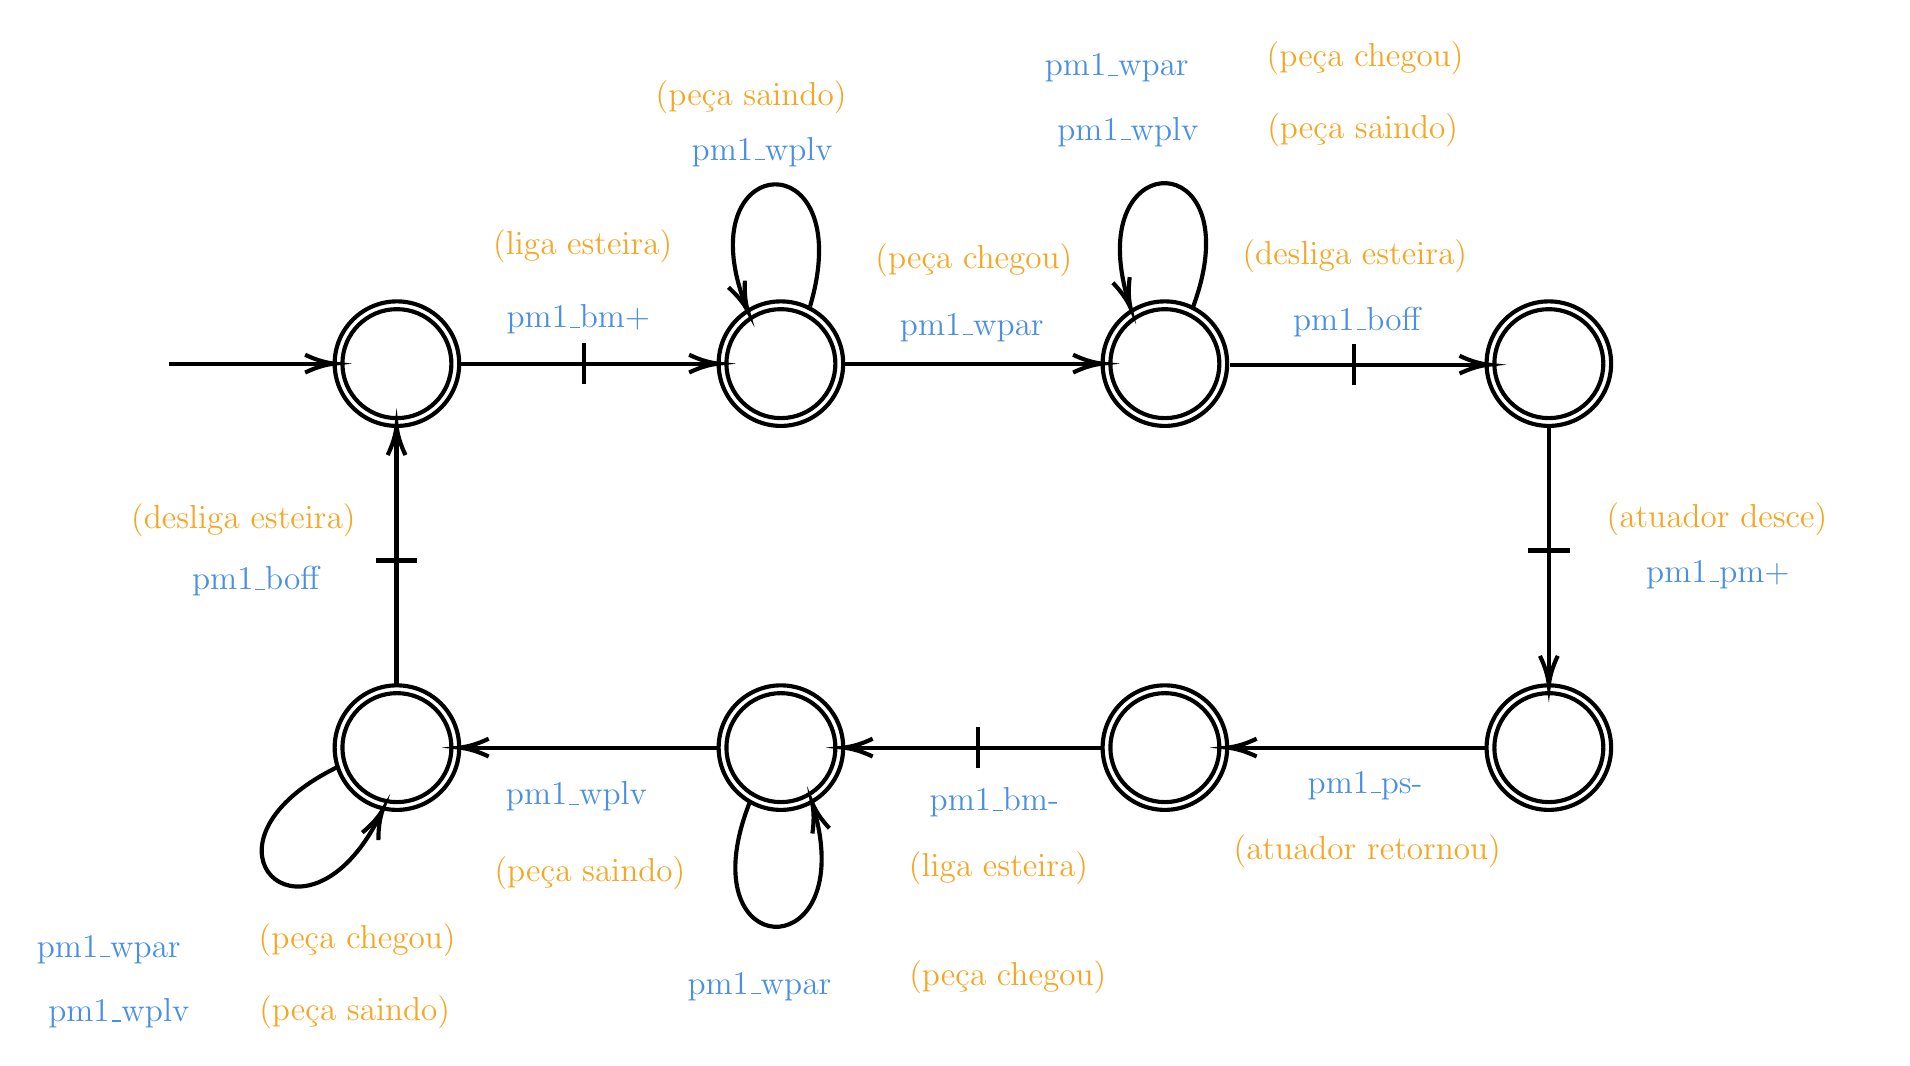
\begin{tikzpicture}[x=0.75pt,y=0.75pt,yscale=-1,xscale=1]
%uncomment if require: \path (0,3420); %set diagram left start at 0, and has height of 3420

%Shape: Circle [id:dp5021231821953818] 
\draw  [line width=1.5]  (1371.5,2916.5) .. controls (1371.5,2899.93) and (1384.93,2886.5) .. (1401.5,2886.5) .. controls (1418.07,2886.5) and (1431.5,2899.93) .. (1431.5,2916.5) .. controls (1431.5,2933.07) and (1418.07,2946.5) .. (1401.5,2946.5) .. controls (1384.93,2946.5) and (1371.5,2933.07) .. (1371.5,2916.5) -- cycle ;
%Shape: Circle [id:dp5289461805073701] 
\draw  [line width=1.5]  (1375.25,2916.5) .. controls (1375.25,2902) and (1387,2890.25) .. (1401.5,2890.25) .. controls (1416,2890.25) and (1427.75,2902) .. (1427.75,2916.5) .. controls (1427.75,2931) and (1416,2942.75) .. (1401.5,2942.75) .. controls (1387,2942.75) and (1375.25,2931) .. (1375.25,2916.5) -- cycle ;
%Straight Lines [id:da4788090574749646] 
\draw [line width=1.5]    (1291.5,2916.5) -- (1368.5,2916.5) ;
\draw [shift={(1371.5,2916.5)}, rotate = 180] [color={rgb, 255:red, 0; green, 0; blue, 0 }  ][line width=1.5]    (14.21,-4.28) .. controls (9.04,-1.82) and (4.3,-0.39) .. (0,0) .. controls (4.3,0.39) and (9.04,1.82) .. (14.21,4.28)   ;
%Straight Lines [id:da8018832314051378] 
\draw [line width=1.5]    (1431.5,2916.5) -- (1454.5,2916.5) -- (1553.5,2916.5) ;
\draw [shift={(1556.5,2916.5)}, rotate = 180] [color={rgb, 255:red, 0; green, 0; blue, 0 }  ][line width=1.5]    (14.21,-4.28) .. controls (9.04,-1.82) and (4.3,-0.39) .. (0,0) .. controls (4.3,0.39) and (9.04,1.82) .. (14.21,4.28)   ;
%Straight Lines [id:da0076803473792970145] 
\draw [line width=1.5]    (1491.5,2906.5) -- (1491.5,2926.5) ;

%Shape: Circle [id:dp22625731925102777] 
\draw  [line width=1.5]  (1556.5,2916.5) .. controls (1556.5,2899.93) and (1569.93,2886.5) .. (1586.5,2886.5) .. controls (1603.07,2886.5) and (1616.5,2899.93) .. (1616.5,2916.5) .. controls (1616.5,2933.07) and (1603.07,2946.5) .. (1586.5,2946.5) .. controls (1569.93,2946.5) and (1556.5,2933.07) .. (1556.5,2916.5) -- cycle ;
%Straight Lines [id:da9270365039391677] 
\draw [line width=1.5]    (1616.5,2916.5) -- (1738.5,2916.5) ;
\draw [shift={(1741.5,2916.5)}, rotate = 180] [color={rgb, 255:red, 0; green, 0; blue, 0 }  ][line width=1.5]    (14.21,-4.28) .. controls (9.04,-1.82) and (4.3,-0.39) .. (0,0) .. controls (4.3,0.39) and (9.04,1.82) .. (14.21,4.28)   ;
%Shape: Circle [id:dp8790830623806889] 
\draw  [line width=1.5]  (1741.5,2916.5) .. controls (1741.5,2899.93) and (1754.93,2886.5) .. (1771.5,2886.5) .. controls (1788.07,2886.5) and (1801.5,2899.93) .. (1801.5,2916.5) .. controls (1801.5,2933.07) and (1788.07,2946.5) .. (1771.5,2946.5) .. controls (1754.93,2946.5) and (1741.5,2933.07) .. (1741.5,2916.5) -- cycle ;
%Shape: Circle [id:dp05996581087867403] 
\draw  [line width=1.5]  (1926.5,2916.5) .. controls (1926.5,2899.93) and (1939.93,2886.5) .. (1956.5,2886.5) .. controls (1973.07,2886.5) and (1986.5,2899.93) .. (1986.5,2916.5) .. controls (1986.5,2933.07) and (1973.07,2946.5) .. (1956.5,2946.5) .. controls (1939.93,2946.5) and (1926.5,2933.07) .. (1926.5,2916.5) -- cycle ;
%Straight Lines [id:da8561532153311397] 
\draw [line width=1.5]    (1956.5,2946.5) -- (1956.5,2969.5) -- (1956.5,3068.5) ;
\draw [shift={(1956.5,3071.5)}, rotate = 270] [color={rgb, 255:red, 0; green, 0; blue, 0 }  ][line width=1.5]    (14.21,-4.28) .. controls (9.04,-1.82) and (4.3,-0.39) .. (0,0) .. controls (4.3,0.39) and (9.04,1.82) .. (14.21,4.28)   ;
%Straight Lines [id:da5406403779740838] 
\draw [line width=1.5]    (1966.5,3006.5) -- (1946.5,3006.5) ;

%Shape: Circle [id:dp1389806805521474] 
\draw  [line width=1.5]  (1926.5,3101.5) .. controls (1926.5,3084.93) and (1939.93,3071.5) .. (1956.5,3071.5) .. controls (1973.07,3071.5) and (1986.5,3084.93) .. (1986.5,3101.5) .. controls (1986.5,3118.07) and (1973.07,3131.5) .. (1956.5,3131.5) .. controls (1939.93,3131.5) and (1926.5,3118.07) .. (1926.5,3101.5) -- cycle ;
%Straight Lines [id:da3566574988633957] 
\draw [line width=1.5]    (1804.5,3101.5) -- (1926.5,3101.5) ;
\draw [shift={(1801.5,3101.5)}, rotate = 0] [color={rgb, 255:red, 0; green, 0; blue, 0 }  ][line width=1.5]    (14.21,-4.28) .. controls (9.04,-1.82) and (4.3,-0.39) .. (0,0) .. controls (4.3,0.39) and (9.04,1.82) .. (14.21,4.28)   ;
%Shape: Circle [id:dp5939143750931828] 
\draw  [line width=1.5]  (1741.5,3101.5) .. controls (1741.5,3084.93) and (1754.93,3071.5) .. (1771.5,3071.5) .. controls (1788.07,3071.5) and (1801.5,3084.93) .. (1801.5,3101.5) .. controls (1801.5,3118.07) and (1788.07,3131.5) .. (1771.5,3131.5) .. controls (1754.93,3131.5) and (1741.5,3118.07) .. (1741.5,3101.5) -- cycle ;
%Shape: Circle [id:dp9635042203289415] 
\draw  [line width=1.5]  (1556.5,3101.5) .. controls (1556.5,3084.93) and (1569.93,3071.5) .. (1586.5,3071.5) .. controls (1603.07,3071.5) and (1616.5,3084.93) .. (1616.5,3101.5) .. controls (1616.5,3118.07) and (1603.07,3131.5) .. (1586.5,3131.5) .. controls (1569.93,3131.5) and (1556.5,3118.07) .. (1556.5,3101.5) -- cycle ;
%Shape: Circle [id:dp022192289610075466] 
\draw  [line width=1.5]  (1371.5,3101.5) .. controls (1371.5,3084.93) and (1384.93,3071.5) .. (1401.5,3071.5) .. controls (1418.07,3071.5) and (1431.5,3084.93) .. (1431.5,3101.5) .. controls (1431.5,3118.07) and (1418.07,3131.5) .. (1401.5,3131.5) .. controls (1384.93,3131.5) and (1371.5,3118.07) .. (1371.5,3101.5) -- cycle ;
%Straight Lines [id:da8665047753384527] 
\draw [line width=1.5]    (1741.5,3101.5) -- (1718.5,3101.5) -- (1619.5,3101.5) ;
\draw [shift={(1616.5,3101.5)}, rotate = 360] [color={rgb, 255:red, 0; green, 0; blue, 0 }  ][line width=1.5]    (14.21,-4.28) .. controls (9.04,-1.82) and (4.3,-0.39) .. (0,0) .. controls (4.3,0.39) and (9.04,1.82) .. (14.21,4.28)   ;
%Straight Lines [id:da33313592666384406] 
\draw [line width=1.5]    (1681.5,3111.5) -- (1681.5,3091.5) ;

%Shape: Circle [id:dp323983994895517] 
\draw  [line width=1.5]  (1560.25,2916.5) .. controls (1560.25,2902) and (1572,2890.25) .. (1586.5,2890.25) .. controls (1601,2890.25) and (1612.75,2902) .. (1612.75,2916.5) .. controls (1612.75,2931) and (1601,2942.75) .. (1586.5,2942.75) .. controls (1572,2942.75) and (1560.25,2931) .. (1560.25,2916.5) -- cycle ;
%Shape: Circle [id:dp061991462662711605] 
\draw  [line width=1.5]  (1745.25,2916.5) .. controls (1745.25,2902) and (1757,2890.25) .. (1771.5,2890.25) .. controls (1786,2890.25) and (1797.75,2902) .. (1797.75,2916.5) .. controls (1797.75,2931) and (1786,2942.75) .. (1771.5,2942.75) .. controls (1757,2942.75) and (1745.25,2931) .. (1745.25,2916.5) -- cycle ;
%Shape: Circle [id:dp8712457883247433] 
\draw  [line width=1.5]  (1930.25,2916.5) .. controls (1930.25,2902) and (1942,2890.25) .. (1956.5,2890.25) .. controls (1971,2890.25) and (1982.75,2902) .. (1982.75,2916.5) .. controls (1982.75,2931) and (1971,2942.75) .. (1956.5,2942.75) .. controls (1942,2942.75) and (1930.25,2931) .. (1930.25,2916.5) -- cycle ;
%Shape: Circle [id:dp4032269267721291] 
\draw  [line width=1.5]  (1930.25,3101.5) .. controls (1930.25,3087) and (1942,3075.25) .. (1956.5,3075.25) .. controls (1971,3075.25) and (1982.75,3087) .. (1982.75,3101.5) .. controls (1982.75,3116) and (1971,3127.75) .. (1956.5,3127.75) .. controls (1942,3127.75) and (1930.25,3116) .. (1930.25,3101.5) -- cycle ;
%Shape: Circle [id:dp7865107563162004] 
\draw  [line width=1.5]  (1745.25,3101.5) .. controls (1745.25,3087) and (1757,3075.25) .. (1771.5,3075.25) .. controls (1786,3075.25) and (1797.75,3087) .. (1797.75,3101.5) .. controls (1797.75,3116) and (1786,3127.75) .. (1771.5,3127.75) .. controls (1757,3127.75) and (1745.25,3116) .. (1745.25,3101.5) -- cycle ;
%Shape: Circle [id:dp6415554207822463] 
\draw  [line width=1.5]  (1560.25,3101.5) .. controls (1560.25,3087) and (1572,3075.25) .. (1586.5,3075.25) .. controls (1601,3075.25) and (1612.75,3087) .. (1612.75,3101.5) .. controls (1612.75,3116) and (1601,3127.75) .. (1586.5,3127.75) .. controls (1572,3127.75) and (1560.25,3116) .. (1560.25,3101.5) -- cycle ;
%Shape: Circle [id:dp25769850815519857] 
\draw  [line width=1.5]  (1375.25,3101.5) .. controls (1375.25,3087) and (1387,3075.25) .. (1401.5,3075.25) .. controls (1416,3075.25) and (1427.75,3087) .. (1427.75,3101.5) .. controls (1427.75,3116) and (1416,3127.75) .. (1401.5,3127.75) .. controls (1387,3127.75) and (1375.25,3116) .. (1375.25,3101.5) -- cycle ;
%Straight Lines [id:da896726859664503] 
\draw [line width=1.5]    (1802.67,2917) -- (1825.67,2917) -- (1924.67,2917) ;
\draw [shift={(1927.67,2917)}, rotate = 180] [color={rgb, 255:red, 0; green, 0; blue, 0 }  ][line width=1.5]    (14.21,-4.28) .. controls (9.04,-1.82) and (4.3,-0.39) .. (0,0) .. controls (4.3,0.39) and (9.04,1.82) .. (14.21,4.28)   ;
%Straight Lines [id:da40191603415797883] 
\draw [line width=1.5]    (1862.67,2907) -- (1862.67,2927) ;

%Straight Lines [id:da303290828710558] 
\draw [line width=1.5]    (1434.5,3101.5) -- (1556.5,3101.5) ;
\draw [shift={(1431.5,3101.5)}, rotate = 0] [color={rgb, 255:red, 0; green, 0; blue, 0 }  ][line width=1.5]    (14.21,-4.28) .. controls (9.04,-1.82) and (4.3,-0.39) .. (0,0) .. controls (4.3,0.39) and (9.04,1.82) .. (14.21,4.28)   ;
%Straight Lines [id:da04070398455869095] 
\draw [line width=1.5]    (1401.33,3071.33) -- (1401.33,3048.33) -- (1401.33,2949.33) ;
\draw [shift={(1401.33,2946.33)}, rotate = 90] [color={rgb, 255:red, 0; green, 0; blue, 0 }  ][line width=1.5]    (14.21,-4.28) .. controls (9.04,-1.82) and (4.3,-0.39) .. (0,0) .. controls (4.3,0.39) and (9.04,1.82) .. (14.21,4.28)   ;
%Straight Lines [id:da6773677195850383] 
\draw [line width=1.5]    (1391.33,3011.33) -- (1411.33,3011.33) ;

%Shape: Boxed Bezier Curve [id:dp5167110010811578] 
\draw [line width=1.5]    (1600.54,2888.94) .. controls (1622.83,2813.24) and (1551.33,2813.02) .. (1565.15,2874.31) .. controls (1566.15,2878.74) and (1567.59,2883.49) .. (1569.55,2888.56) ;
\draw [shift={(1570.63,2891.27)}, rotate = 247.54] [color={rgb, 255:red, 0; green, 0; blue, 0 }  ][line width=1.5]    (14.21,-4.28) .. controls (9.04,-1.82) and (4.3,-0.39) .. (0,0) .. controls (4.3,0.39) and (9.04,1.82) .. (14.21,4.28)   ;
%Shape: Boxed Bezier Curve [id:dp9243950747298513] 
\draw [line width=1.5]    (1784.98,2889.43) .. controls (1812.53,2815.49) and (1741.22,2810.25) .. (1750.7,2872.35) .. controls (1751.38,2876.84) and (1752.49,2881.68) .. (1754.09,2886.87) ;
\draw [shift={(1754.98,2889.66)}, rotate = 251.57] [color={rgb, 255:red, 0; green, 0; blue, 0 }  ][line width=1.5]    (14.21,-4.28) .. controls (9.04,-1.82) and (4.3,-0.39) .. (0,0) .. controls (4.3,0.39) and (9.04,1.82) .. (14.21,4.28)   ;
%Shape: Boxed Bezier Curve [id:dp87649693826674] 
\draw [line width=1.5]    (1372.77,3110.91) .. controls (1301.92,3145.65) and (1350.09,3198.49) .. (1385.91,3146.88) .. controls (1388.5,3143.15) and (1391.03,3138.87) .. (1393.44,3134) ;
\draw [shift={(1394.71,3131.37)}, rotate = 115.01] [color={rgb, 255:red, 0; green, 0; blue, 0 }  ][line width=1.5]    (14.21,-4.28) .. controls (9.04,-1.82) and (4.3,-0.39) .. (0,0) .. controls (4.3,0.39) and (9.04,1.82) .. (14.21,4.28)   ;
%Shape: Boxed Bezier Curve [id:dp13960413507575198] 
\draw [line width=1.5]    (1571.55,3127.67) .. controls (1542.5,3201.03) and (1613.69,3207.72) .. (1605.47,3145.44) .. controls (1604.88,3140.93) and (1603.87,3136.07) .. (1602.38,3130.85) ;
\draw [shift={(1601.54,3128.05)}, rotate = 72.73] [color={rgb, 255:red, 0; green, 0; blue, 0 }  ][line width=1.5]    (14.21,-4.28) .. controls (9.04,-1.82) and (4.3,-0.39) .. (0,0) .. controls (4.3,0.39) and (9.04,1.82) .. (14.21,4.28)   ;

% Text Node
\draw (1488.5,2891.5) node  [font=\large] [align=left] {\begin{minipage}[lt]{51.17pt}\setlength\topsep{0pt}
\begin{center}
\textcolor[rgb]{0.29,0.56,0.89}{pm1\_bm+}
\end{center}

\end{minipage}};
% Text Node
\draw (1491,2860) node  [font=\large] [align=left] {\begin{minipage}[lt]{94.73pt}\setlength\topsep{0pt}
\begin{center}
\textcolor[rgb]{0.96,0.65,0.14}{(liga esteira)}
\end{center}

\end{minipage}};
% Text Node
\draw (1678,2895) node  [font=\large] [align=left] {\begin{minipage}[lt]{51.17pt}\setlength\topsep{0pt}
\begin{center}
\textcolor[rgb]{0.29,0.56,0.89}{pm1\_wpar}
\end{center}

\end{minipage}};
% Text Node
\draw (1679.5,2866.5) node  [font=\large] [align=left] {\begin{minipage}[lt]{98.81pt}\setlength\topsep{0pt}
\begin{center}
\textcolor[rgb]{0.96,0.65,0.14}{(peça chegou)}
\end{center}

\end{minipage}};
% Text Node
\draw (1864,2896.5) node  [font=\large] [align=left] {\begin{minipage}[lt]{58.23pt}\setlength\topsep{0pt}
\begin{center}
\textcolor[rgb]{0.29,0.56,0.89}{pm1\_boff}
\end{center}

\end{minipage}};
% Text Node
\draw (1863,2865) node  [font=\large] [align=left] {\begin{minipage}[lt]{98.81pt}\setlength\topsep{0pt}
\begin{center}
\textcolor[rgb]{0.96,0.65,0.14}{(desliga esteira)}
\end{center}

\end{minipage}};
% Text Node
\draw (1868,3120) node  [font=\large] [align=left] {\begin{minipage}[lt]{57.55pt}\setlength\topsep{0pt}
\begin{center}
\textcolor[rgb]{0.29,0.56,0.89}{pm1\_ps-}
\end{center}

\end{minipage}};
% Text Node
\draw (1869,3151.5) node  [font=\large] [align=left] {\begin{minipage}[lt]{112.65pt}\setlength\topsep{0pt}
\begin{center}
\textcolor[rgb]{0.96,0.65,0.14}{(atuador retornou)}
\end{center}

\end{minipage}};
% Text Node
\draw (2038,3018.33) node  [font=\large] [align=left] {\begin{minipage}[lt]{57.55pt}\setlength\topsep{0pt}
\begin{center}
\textcolor[rgb]{0.29,0.56,0.89}{pm1\_pm+}
\end{center}

\end{minipage}};
% Text Node
\draw (2037.5,2991.33) node  [font=\large] [align=left] {\begin{minipage}[lt]{112.65pt}\setlength\topsep{0pt}
\begin{center}
\textcolor[rgb]{0.96,0.65,0.14}{(atuador desce)}
\end{center}

\end{minipage}};
% Text Node
\draw (1689.33,3128) node  [font=\large] [align=left] {\begin{minipage}[lt]{57.55pt}\setlength\topsep{0pt}
\begin{center}
\textcolor[rgb]{0.29,0.56,0.89}{pm1\_bm-}
\end{center}

\end{minipage}};
% Text Node
\draw (1691.33,3159.5) node  [font=\large] [align=left] {\begin{minipage}[lt]{112.65pt}\setlength\topsep{0pt}
\begin{center}
\textcolor[rgb]{0.96,0.65,0.14}{(liga esteira)}
\end{center}

\end{minipage}};
% Text Node
\draw (1488,3125) node  [font=\large] [align=left] {\begin{minipage}[lt]{57.55pt}\setlength\topsep{0pt}
\begin{center}
\textcolor[rgb]{0.29,0.56,0.89}{pm1\_wplv}
\end{center}

\end{minipage}};
% Text Node
\draw (1494.5,3162) node  [font=\large] [align=left] {\begin{minipage}[lt]{112.65pt}\setlength\topsep{0pt}
\begin{center}
\textcolor[rgb]{0.96,0.65,0.14}{(peça saindo)}
\end{center}

\end{minipage}};
% Text Node
\draw (1333.5,3021.5) node  [font=\large] [align=left] {\begin{minipage}[lt]{57.55pt}\setlength\topsep{0pt}
\begin{center}
\textcolor[rgb]{0.29,0.56,0.89}{pm1\_boff}
\end{center}

\end{minipage}};
% Text Node
\draw (1327.5,2992) node  [font=\large] [align=left] {\begin{minipage}[lt]{112.65pt}\setlength\topsep{0pt}
\begin{center}
\textcolor[rgb]{0.96,0.65,0.14}{(desliga esteira)}
\end{center}

\end{minipage}};
% Text Node
\draw (1577.5,2814.5) node  [font=\large] [align=left] {\begin{minipage}[lt]{57.55pt}\setlength\topsep{0pt}
\begin{center}
\textcolor[rgb]{0.29,0.56,0.89}{pm1\_wplv}
\end{center}

\end{minipage}};
% Text Node
\draw (1572.17,2788) node  [font=\large] [align=left] {\begin{minipage}[lt]{112.65pt}\setlength\topsep{0pt}
\begin{center}
\textcolor[rgb]{0.96,0.65,0.14}{(peça saindo)}
\end{center}

\end{minipage}};
% Text Node
\draw (1753.67,2805) node  [font=\large] [align=left] {\begin{minipage}[lt]{57.55pt}\setlength\topsep{0pt}
\begin{center}
\textcolor[rgb]{0.29,0.56,0.89}{pm1\_wplv}
\end{center}

\end{minipage}};
% Text Node
\draw (1866.83,2804) node  [font=\large] [align=left] {\begin{minipage}[lt]{112.65pt}\setlength\topsep{0pt}
\begin{center}
\textcolor[rgb]{0.96,0.65,0.14}{(peça saindo)}
\end{center}

\end{minipage}};
% Text Node
\draw (1747.83,2770) node  [font=\large] [align=left] {\begin{minipage}[lt]{51.17pt}\setlength\topsep{0pt}
\begin{center}
\textcolor[rgb]{0.29,0.56,0.89}{pm1\_wpar}
\end{center}

\end{minipage}};
% Text Node
\draw (1868,2769.5) node  [font=\large] [align=left] {\begin{minipage}[lt]{98.81pt}\setlength\topsep{0pt}
\begin{center}
\textcolor[rgb]{0.96,0.65,0.14}{(peça chegou)}
\end{center}

\end{minipage}};
% Text Node
\draw (1267.5,3229.5) node  [font=\large] [align=left] {\begin{minipage}[lt]{57.55pt}\setlength\topsep{0pt}
\begin{center}
\textcolor[rgb]{0.29,0.56,0.89}{pm1\_wplv}
\end{center}

\end{minipage}};
% Text Node
\draw (1381.17,3228.83) node  [font=\large] [align=left] {\begin{minipage}[lt]{112.65pt}\setlength\topsep{0pt}
\begin{center}
\textcolor[rgb]{0.96,0.65,0.14}{(peça saindo)}
\end{center}

\end{minipage}};
% Text Node
\draw (1262.17,3194.83) node  [font=\large] [align=left] {\begin{minipage}[lt]{51.17pt}\setlength\topsep{0pt}
\begin{center}
\textcolor[rgb]{0.29,0.56,0.89}{pm1\_wpar}
\end{center}

\end{minipage}};
% Text Node
\draw (1382.33,3194.33) node  [font=\large] [align=left] {\begin{minipage}[lt]{98.81pt}\setlength\topsep{0pt}
\begin{center}
\textcolor[rgb]{0.96,0.65,0.14}{(peça chegou)}
\end{center}

\end{minipage}};
% Text Node
\draw (1575.67,3212.67) node  [font=\large] [align=left] {\begin{minipage}[lt]{51.17pt}\setlength\topsep{0pt}
\begin{center}
\textcolor[rgb]{0.29,0.56,0.89}{pm1\_wpar}
\end{center}

\end{minipage}};
% Text Node
\draw (1695.83,3212.17) node  [font=\large] [align=left] {\begin{minipage}[lt]{98.81pt}\setlength\topsep{0pt}
\begin{center}
\textcolor[rgb]{0.96,0.65,0.14}{(peça chegou)}
\end{center}

\end{minipage}};


\end{tikzpicture}}
        \caption{Restrição para PM1.}
        \label{fig:H_PM1}
    \end{figure}

\end{frame}

 
\section{Conclusão}

\begin{frame}{Concluindo}

É possível concluir que obteve-se exito em controlar a planta proposta pelo grupo, através da simulação nos \textit{softwares} foi possível visualizar seu funcionamento conforme desejado inicialmente, com as duas saídas intercaladas de milkshake e as restrições aplicadas.

\vspace{0.5cm}
O sistema resultante também é não bloqueante, de forma que não apresenta situações com \textit{livelock} ou \textit{deadlock}.


%funcionou e o sistema é não bloqueante

\end{frame} 

\backmatter

\bibliographystyle{plain}
\bibliography{ref.bib}
\end{document}
